\documentclass[12pt, border=12pt]{standalone}
\usepackage[utf8]{inputenc}
\usepackage[utf8]{vietnam}
\usepackage{amsmath,amsfonts,amssymb}
\usepackage{type1cm}
\usepackage{graphicx}
\usepackage{multirow}
\usepackage{multicol}
\usepackage{array}
\usepackage{comment}
\usepackage[unicode]{hyperref}
\usepackage{tikz}
\usepackage{color}
\usepackage[american,cuteinductors,smartlabels]{circuitikz}
\usetikzlibrary{arrows}
\usepackage{tikz}
\usetikzlibrary{calc,patterns,angles,quotes}
\usetikzlibrary{arrows, decorations.markings, calc, fadings, decorations.pathreplacing, patterns, decorations.pathmorphing, positioning}	
%\tikzstyle{every path}=[line width=1.2pt]

\tikzset{middlearrow/.style={
        decoration={markings,
            mark= at position 0.5 with {\arrow{#1}} ,
        },
        postaction={decorate}
    }
}
\begin{document}
	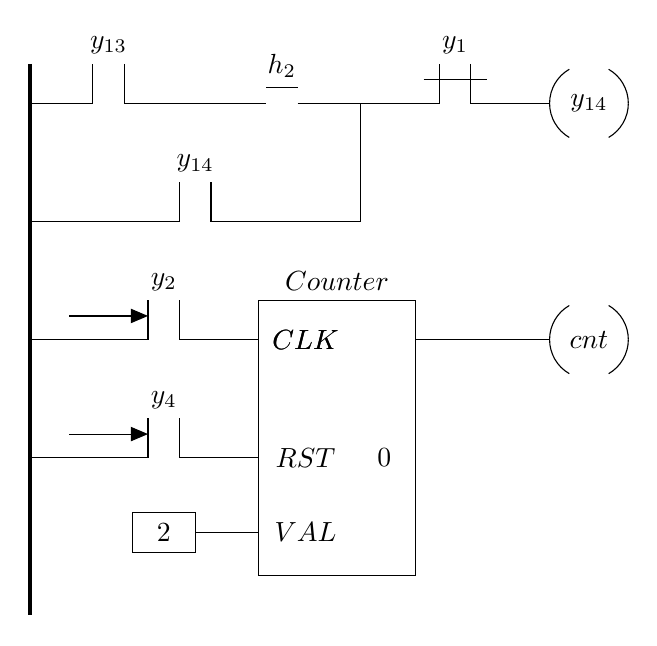
\begin{tikzpicture}[>=triangle 45]
		\draw[ultra thick] (8.5,-17.5) -- (8.5,-24.5);
				
		\draw (8.5,-18) -- (9.3,-18) -- (9.3,-17.5); \draw (9.7,-17.5) -- (9.7,-18) -- (11.5,-18); \draw (9.5,-17.5) node[above]{$y_{13}$};  \draw (11.5,-17.8) -- (11.9,-17.8); \draw(11.7,-17.8) node[above]{$h_2$}; \draw (11.9,-18) -- (12.7,-18); \draw (12.7,-18) -- (13.7,-18)-- (13.7,-17.5); \draw (14.1,-17.5) -- (14.1,-18)-- (15.1,-18); \draw (13.5,-17.7) -- (14.3, -17.7); \draw (13.9,-17.5) node[above]{$y_{1}$};  \draw (15.1,-18) arc (180:120:.5);\draw (15.1,-18) arc (180:240:.5); \draw (16.1,-18) arc (0:60:.5);\draw (16.1,-18) arc (0:-60:.5); \draw (15.6,-18) node{$y_{14}$}; \draw (8.5,-19.5) -- (10.4,-19.5) -- (10.4,-19); \draw (10.8,-19) -- (10.8,-19.5)  -- (12.7,-19.5) -- (12.7,-18); \draw (10.6,-19) node[above]{$y_{14}$}; 
						
		\draw (8.5,-21) -- (10,-21) -- (10,-20.5); \draw (10.4,-20.5) -- (10.4,-21) -- (11.4,-21);  \draw[->] (9,-20.7) -- (10,-20.7); \draw (10.2,-20.5) node[above]{$y_2$}; \draw (12,-21) node {$CLK$}; \draw (11.4,-20.5) rectangle (13.4,-24); \draw (8.5,-22.5) -- (10,-22.5) -- (10,-22); \draw (10.4,-22) -- (10.4,-22.5) -- (11.4,-22.5); \draw[->] (9,-22.2) -- (10,-22.2); \draw (10.2,-22) node[above]{$y_4$}; \draw (12,-22.5) node {$RST$}; \draw (13,-22.5) node {$0$};\draw (9.8,-23.2) rectangle (10.6,-23.7); \draw (10.2,-23.45) node{$2$}; \draw (10.6,-23.45) -- (11.4,-23.45); \draw (12,-23.45) node {$VAL$}; \draw (12,-21) node {$CLK$}; \draw (12.4,-20.5) node[above] {$Counter$}; \draw (13.4,-21) -- (15.1,-21); \draw (15.1,-21) arc (180:120:.5);\draw (15.1,-21) arc (180:240:.5); \draw (16.1,-21) arc (0:60:.5);\draw (16.1,-21) arc (0:-60:.5); \draw (15.6,-21) node{$cnt$};
	\end{tikzpicture}
\end{document}